%%%%%%%%%%%%%%%%%%%%%%%%%%%%%%%%%%%%%%%%%%%%%%%%%%%%%%%%%%%%%%%%%%%%%%
% Overleaf (WriteLaTeX) Example: Molecular Chemistry Presentation
%
% Source: http://www.overleaf.com
%
% In these slides we show how Overleaf can be used with standard 
% chemistry packages to easily create professional presentations.
% 
% Feel free to distribute this example, but please keep the referral
% to overleaf.com
% 
%%%%%%%%%%%%%%%%%%%%%%%%%%%%%%%%%%%%%%%%%%%%%%%%%%%%%%%%%%%%%%%%%%%%%%

\documentclass{beamer}

\mode<presentation>
{
  \usetheme{Madrid}       % or try default, Darmstadt, Warsaw, ...
  \usecolortheme{default} % or try albatross, beaver, crane, ...
  \usefonttheme{default}    % or try default, structurebold, ...
  \setbeamertemplate{navigation symbols}{}
  \setbeamertemplate{caption}[numbered]
} 

\usepackage[english]{babel}
\usepackage[utf8x]{inputenc}
\usepackage{graphicx}
\usepackage{hyperref}
  \hypersetup{colorlinks=true}
  \hypersetup{urlcolor=blue}
  \hypersetup{linkcolor = .}
\usepackage{xcolor}
\usepackage{siunitx}
  \sisetup{separate-uncertainty = true}
\usepackage{physics}
\usepackage[font=small,labelfont=bf]{caption}
\usepackage{subcaption}
\usepackage[en-GB]{datetime2}
\usepackage{overpic}
\usepackage{feynmp}
\DeclareGraphicsRule{*}{mps}{*}{}
\usepackage{scalerel}
\newcommand{\mylbrace}[2]{\vspace{#2pt}\hspace{6pt}\scaleleftright[\dimexpr5pt+#1\dimexpr0.06pt]{\lbrace}{\rule[\dimexpr2pt-#1\dimexpr0.5pt]{-4pt}{#1pt}}{.}}
\newcommand{\myrbrace}[2]{\vspace{#2pt}\scaleleftright[\dimexpr5pt+#1\dimexpr0.06pt]{.}{\rule[\dimexpr2pt-#1\dimexpr0.5pt]{-4pt}{#1pt}}{\rbrace}\hspace{6pt}}

% Trim in percent
\usepackage{adjustbox}

% No "Figure" prefix
\setbeamertemplate{caption}{\raggedright\insertcaption\par}

% Nice decay amplitude diagrams
\usepackage{amsmath,amssymb,tikz-cd}

% Strike out text
\usepackage[normalem]{ulem}

% For figures with text overlay
\usepackage{overpic}

% Here's where the presentation starts, with the info for the title slide
\title[$B^\pm\to{[K^+K^-\pi^+\pi^-]}_Dh^\pm$]{Model independent measurement of the CKM angle \texorpdfstring{$\gamma$}{gamma} with \texorpdfstring{$B^\pm\to[K^+K^-\pi^+\pi^-]_Dh^\pm$}{B2DhD2KKpipi} at LHCb and BESIII}

\author{Martin Tat}
\institute[University of Oxford]{\normalsize University of Oxford\\ \vspace{0.3cm}\normalsize IOP Joint APP and HEPP Conference}
\date{3rd-5th April 2023}

\titlegraphic{
\includegraphics[height = 2cm]{lhcb.jpg}\hspace{1cm}~%
              
\includegraphics[height = 2cm]{OxfordLogo.pdf}\hspace{1cm}~%
              
\includegraphics[height = 2cm]{bes3.jpg}}

\begin{document}

\begin{frame}
  \titlepage
\end{frame}

% These three lines create an automatically generated table of contents.
% \begin{frame}{Outline}
%   \tableofcontents
% \end{frame}

\section{Introduction to \texorpdfstring{$\gamma$}{gamma} and \texorpdfstring{$C\!P$}{CP} violation}
\begin{frame}{Introduction to $\gamma$ and $C\!P$ violation}
  \begin{center}
    {\huge Introduction to $\gamma$ and $C\!P$ violation}
  \end{center}
\end{frame}

\begin{frame}{Introduction to $\gamma$ and $C\!P$ violation}
  \begin{itemize}
    \setlength\itemsep{0.3em}
    \item{CPV in SM is described by the Unitary Triangle, with angles $\alpha$, $\beta$, $\gamma$}
    \item{The angle $\gamma = \text{arg}\Big(-\frac{V^{\phantom{*}}_{ud}V^*_{ub}}{V^{\phantom{*}}_{cd}V^*_{cb}}\Big)$ is very important:}
    \begin{enumerate}
    \setlength\itemsep{0.2em}
      \item{Negligible theoretical uncertainties: Ideal SM benchmark}
      \item{Accessible at tree level: Indirectly probe New Physics that enter loops}
      \item{Compare with $\alpha$, $\beta$ measurements: Is the Unitary Triangle a triangle?}
    \end{enumerate}
  \end{itemize}
  \vspace{-0.2cm}
  \begin{figure}
    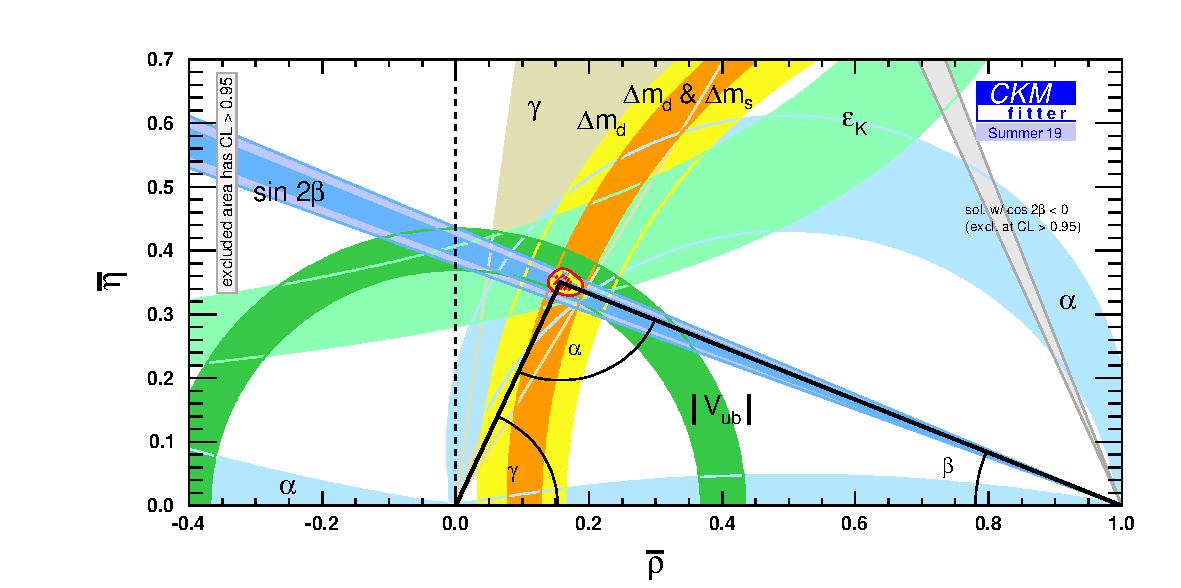
\includegraphics[width = 0.70\textwidth]{Plots/ckmfitter2.pdf}
    \vspace{-0.3cm}
    \caption*{\tiny CKMfitter Group (J. Charles et al.), Eur. Phys. J. C41, 1-131 (2005)}
  \end{figure}
\end{frame}

\begin{frame}{Sensitivity through interference}
  \begin{center}
    \Large Measure $\gamma$ through interference effects in $B^\pm\to DK^\pm$
  \end{center}
  \begin{figure}[H]
    \centering
    \begin{subfigure}{0.5\textwidth}
      \centering
      \begin{fmffile}{fgraph/fgraph_BtoDK1}
        \setlength{\unitlength}{0.4cm}
        \begin{fmfgraph*}(6,6)
          \fmfstraight
          \fmfleft{i1,B,i2,t1,t2,t3,t9,t10}
          \fmfright{o1,D,o2,t4,t5,o3,K,o4}
          \fmflabel{$\bar{u}$}{i1}
          \fmflabel{$b$}{i2}
          \fmfv{l.d=20,l.a=180,l={$B^-$\mylbrace{30}{-8}}}{B}
          \fmflabel{$\bar{u}$}{o1}
          \fmflabel{$c$}{o2}
          \fmflabel{$\bar{u}$}{o3}
          \fmflabel{$s$}{o4}
          \fmfv{l.d=15,l.a=0,l={\myrbrace{30}{-12}}$D^0$}{D}
          \fmfv{l.d=15,l.a=0,l={\myrbrace{30}{11}}$K^-$}{K}
          \fmf{fermion}{o1,i1}
          \fmf{fermion,tension=1.5}{i2,v1}
          \fmf{fermion}{v1,o2}
          \fmf{phantom,tension=1.5}{t9,v2}
          \fmf{boson,label=$W$,label.side=left,tension=0}{v1,v2}
          \fmf{fermion}{v2,o4}
          \fmf{fermion}{o3,v2}
        \end{fmfgraph*}
      \end{fmffile}
      \vspace{0.5cm}
      \caption*{Favoured $B^-\to D^0K^-$}
    \end{subfigure}%
    \begin{subfigure}{0.5\textwidth}
      \centering
      \begin{fmffile}{fgraph/fgraph_BtoDK2}
        \setlength{\unitlength}{0.4cm}
        \begin{fmfgraph*}(6,6)
          \fmfstraight
          \fmfleft{i1,t1,t2,B,t9,t10,i2}
          \fmfright{o1,K,o2,t4,t5,o3,D,o4}
          \fmflabel{$\bar{u}$}{i1}
          \fmflabel{$b$}{i2}
          \fmfv{l.d=20,l.a=180,l={$B^-$\mylbrace{100}{-8}}}{B}
          \fmflabel{$\bar{u}$}{o1}
          \fmflabel{$s$}{o2}
          \fmflabel{$\bar{c}$}{o3}
          \fmflabel{$u$}{o4}
          \fmfv{l.d=15,l.a=0,l={\myrbrace{30}{13}}$\bar{D^0}$}{D}
          \fmfv{l.d=15,l.a=0,l={\myrbrace{30}{-13}}$K^-$}{K}
          \fmf{fermion}{o1,i1}
          \fmf{fermion,tension=1.5}{i2,v1}
          \fmf{fermion}{v1,o4}
          \fmf{phantom,tension=1.5}{t2,v2}
          \fmf{boson,label=$W$,label.side=left,tension=0}{v1,v2}
          \fmf{fermion}{v2,o2}
          \fmf{fermion}{o3,v2}
        \end{fmfgraph*}
      \end{fmffile}
      \vspace{0.5cm}
      \caption*{Suppressed $B^-\to\bar{D^0}K^-$}
    \end{subfigure}
  \end{figure}
  \vspace{-0.3cm}
  \begin{itemize}
    \item{Superposition of $D^0$ and $\bar{D^0}$}
    \item{$b\to u\bar{c}s$ and $b\to c\bar{u}s$ interference $\to$ Sensitivity to $\gamma$}
  \end{itemize}
  \vspace{-0.3cm}
  \begin{center}
    $\mathcal{A}(B^-)=\mathcal{A}_B\Big(\mathcal{A}_{D^0} + r_Be^{i(\delta_B - \gamma)}\mathcal{A}_{\bar{D^0}}\Big)$ \\
    $\mathcal{A}(B^+)=\mathcal{A}_B\Big(\mathcal{A}_{\bar{D^0}} + r_Be^{i(\delta_B + \gamma)}\mathcal{A}_{D^0}\Big)$ \\
  \end{center}
  \vspace{-0.3cm}
  \begin{itemize}
    \item{The magnitude of interference effects governed by $r_B\approx0.1$}
  \end{itemize}
\end{frame}

\begin{frame}[fragile]{Sensitivity through interference}
  \begin{center}
    Phase space integrated analysis: Compare yields of $B^+$ and $B^-$\\~\\
    Interference depends on $\gamma$, but it is diluted by $\kappa$ when integrated over phase space
  \end{center}
  \begin{equation*}
    \begin{tikzcd}[column sep=huge]
      & D^0K^- \arrow[dr, bend left = 25, "\mathcal{A}_{D^0}"] & \\
      B^- \arrow[ur, bend left, "\mathcal{A}_B"] \arrow[dr, bend right, "\mathcal{A}_B r_B e^{i(\delta_B - \gamma)}"'] & [5cm] & DK^- \\
      & \bar{D^0}K^- \arrow[ur, bend right = 25, "\mathcal{A}_{\bar{D^0}}"'] & \\
    \end{tikzcd}
  \end{equation*}
  \begin{equation*}
    \lvert\mathcal{A}(B^-)\lvert^2\propto1 + r_B^2 + 2r_B\kappa\cos(\delta_B - \gamma)
  \end{equation*}
\end{frame}

\begin{frame}{First look at $B^\pm\to[K^+K^-\pi^+\pi^-]_DK^\pm$}
  \begin{figure}
    \centering
    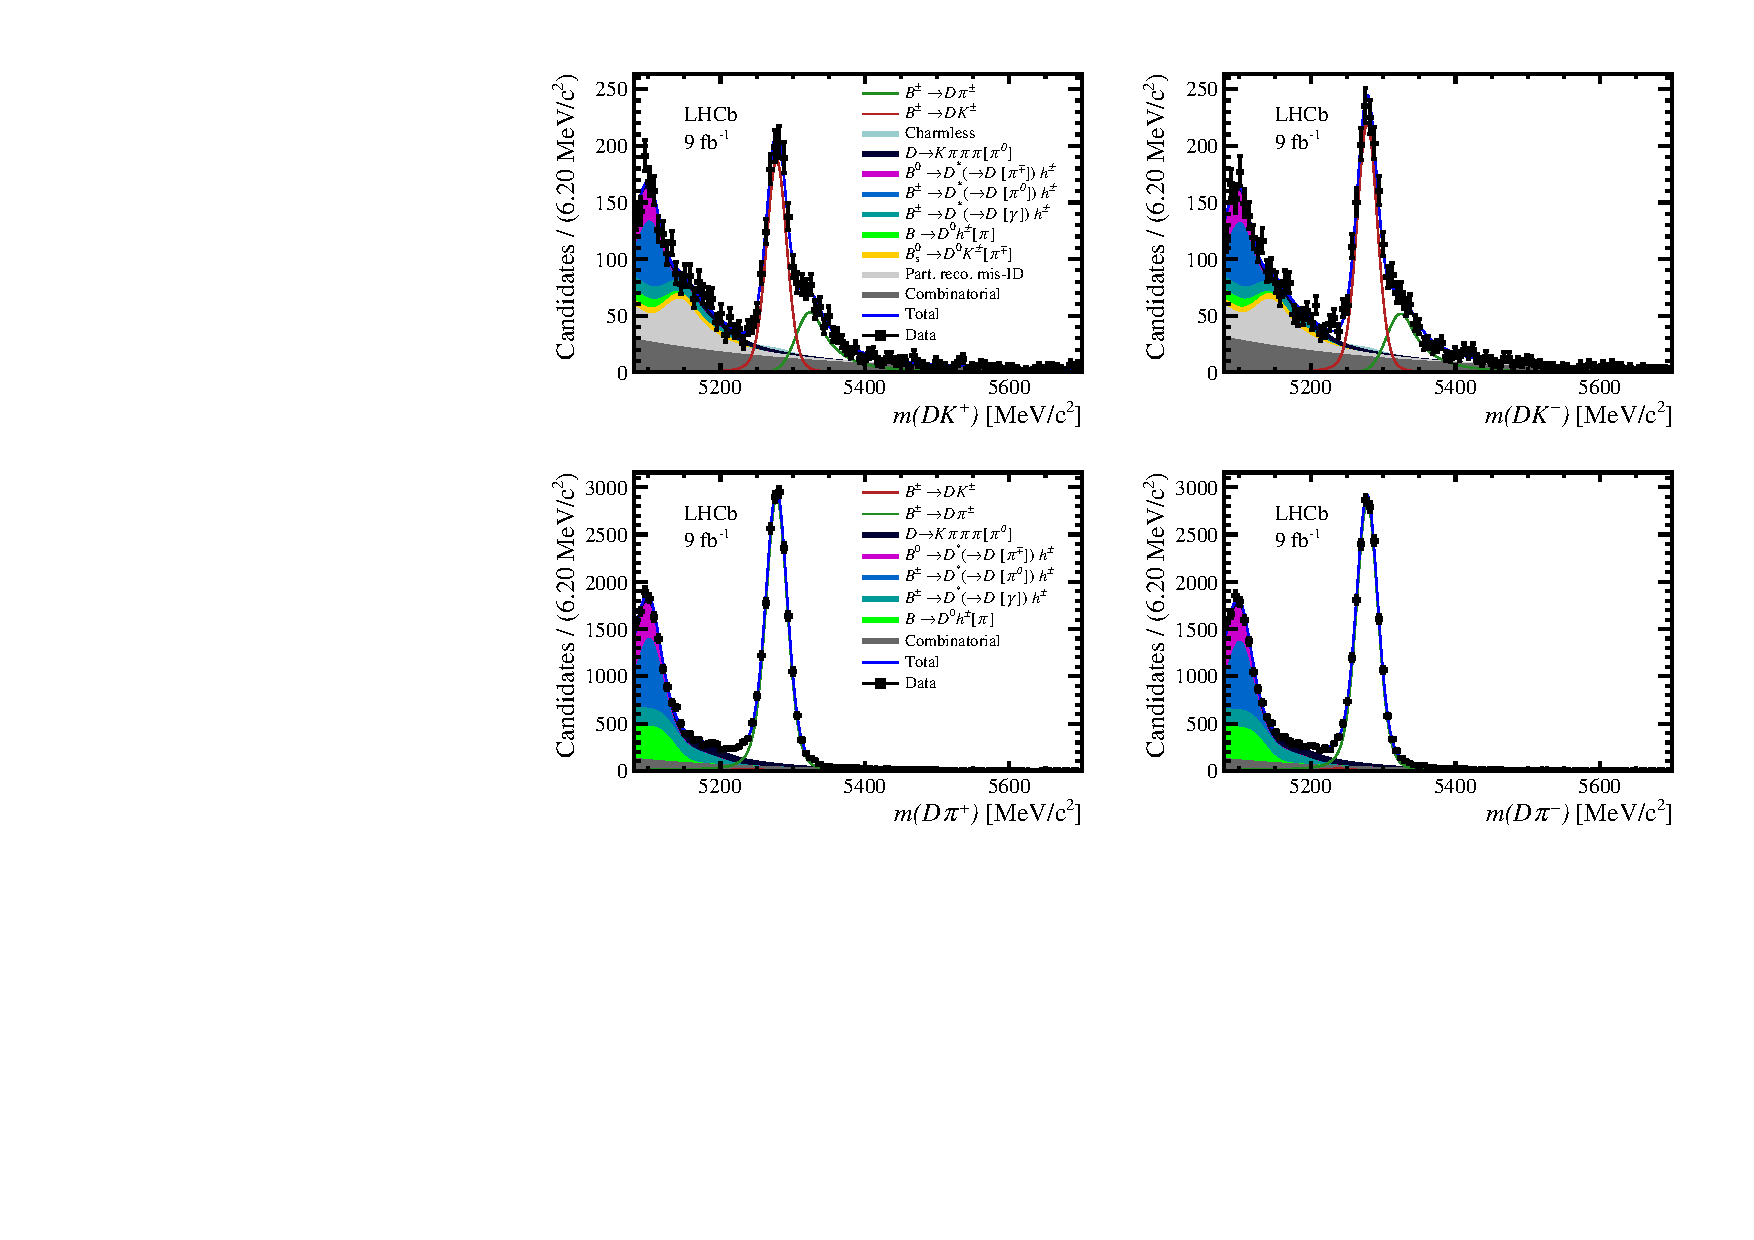
\includegraphics[width = 1.0\textwidth]{Plots/d2kkpipi_fiveL_allDP_GLW.pdf}
    \caption*{\tiny arXiv:2301.10328}
  \end{figure}
  \vspace{-0.5cm}
  \begin{center}
    \Large Clear asymmetry due to $C\!P$ violation
  \end{center}
\end{frame}

\begin{frame}{First look at $B^\pm\to[K^+K^-\pi^+\pi^-]_DK^\pm$}
  \begin{equation*}
    \mathcal{A} = \frac{2r_B\kappa\sin(\delta_B)\sin(\gamma)}{1 + r_B^2 + 2r_B\kappa\cos(\delta_B)\cos(\gamma)}
  \end{equation*}
  \begin{center}
    {\large Measuring the $B^\pm\to DK^\pm$ asymmetry $\mathcal{A}$ provide useful constraints on $\gamma$, but with some caveats:}
  \end{center}
  \begin{enumerate}
    \item{Interference effects are diluted by a factor $\kappa = \SI{0.46(8)}{}$}
    \begin{itemize}
      \item{Phys. Rev. D \textbf{107}, 032009}
    \end{itemize}
    \item{Second order sensitivity to $\cos(\gamma)$}
    \item{Four-fold symmetry:}
    \begin{itemize}
      \item{$(\gamma, \delta_B)\to(\delta_B, \gamma)$}
      \item{$(\gamma, \delta_B)\to(\pi - \gamma, \pi - \delta_B)$}
    \end{itemize}
  \end{enumerate}
  \begin{center}
    \Large Solution: Perform analysis in local regions of phase space!
  \end{center}
\end{frame}

\section{Phase space binned analysis of \texorpdfstring{$B^\pm\to[K^+K^-\pi^+\pi^-]_DK^\pm$}{B2DKD2KKpipi}}
\begin{frame}{Phase space binned analysis of $B^\pm\to[K^+K^-\pi^+\pi^-]_DK^\pm$}
  \begin{center}
    {\huge Phase space binned analysis of $B^\pm\to[K^+K^-\pi^+\pi^-]_DK^\pm$}
  \end{center}
\end{frame}

\begin{frame}{Phase space binned analysis of $B^\pm\to[K^+K^-\pi^+\pi^-]_DK^\pm$}
  \begin{center}
    \Large First study of $C\!P$ violation in $B^\pm\to[K^+K^-\pi^+\pi^-]_DK^\pm$\\~\\
  \end{center}
  \begin{itemize}
    \setlength\itemsep{1.0em}
    \item{Proposed by J. Rademacker and G. Wilkinson}
    \begin{itemize}
      \item{Phys. Lett. \textbf{B647} (2007) 400}
      \item{FOCUS amplitude model predicts a $14^\circ$ precision with $1000$ candidates}
    \end{itemize}
    \item{State of the art amplitude analysis by LHCb:}
    \begin{itemize}
      \item{JHEP \textbf{02} (2019) 126}
      \item{Exploits the huge dataset of charm decays collected by LHCb}
    \end{itemize}
    \item{Large interference effects in local regions of the 5D phase space}
    \begin{itemize}
      \item{Identify regions with similar asymmetries and split into bins}
    \end{itemize}
  \end{itemize}
\end{frame}

\begin{frame}{Phase space binned analysis of $B^\pm\to[K^+K^-\pi^+\pi^-]_DK^\pm$}
  \begin{itemize}
    \setlength\itemsep{1.0em}
    \item{Analogous to the decays $D^0\to K_S^0\pi^+\pi^-$ and $K_S^0K^+K^-$, where the binning scheme may be visualised on a Dalitz plot}
  \end{itemize}
  \begin{figure}
    \begin{subfigure}{0.45\textwidth}
      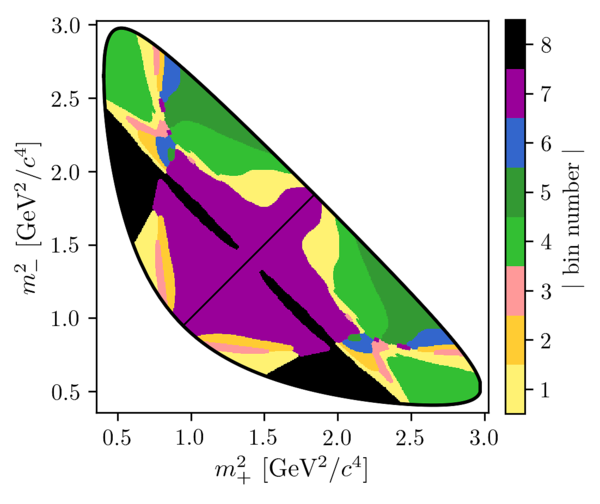
\includegraphics[height = 4cm]{Plots/KsPiPi_optimal.png}
      \caption*{$K_S^0\pi^+\pi^-$}
    \end{subfigure}%
    \begin{subfigure}{0.45\textwidth}
      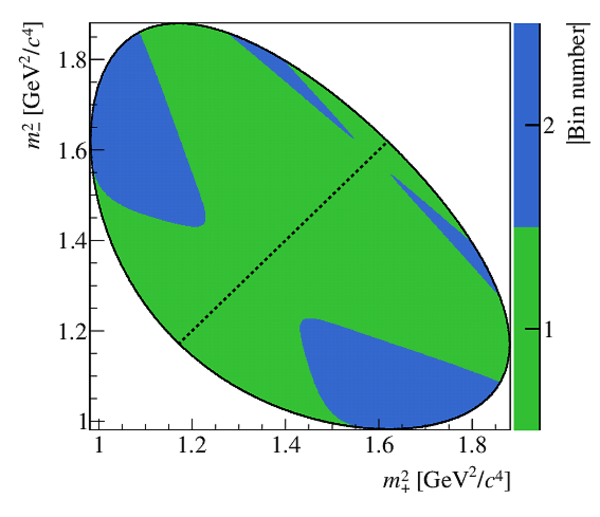
\includegraphics[height = 4cm]{Plots/KsKK_binning.png}
      \caption*{$K_S^0K^+K^-$}
    \end{subfigure}
  \end{figure}
\end{frame}

\begin{frame}{Binned analysis of the $D\to K^+K^-\pi^+\pi^-$ mode}
  \begin{figure}
    \begin{subfigure}{0.5\textwidth}
      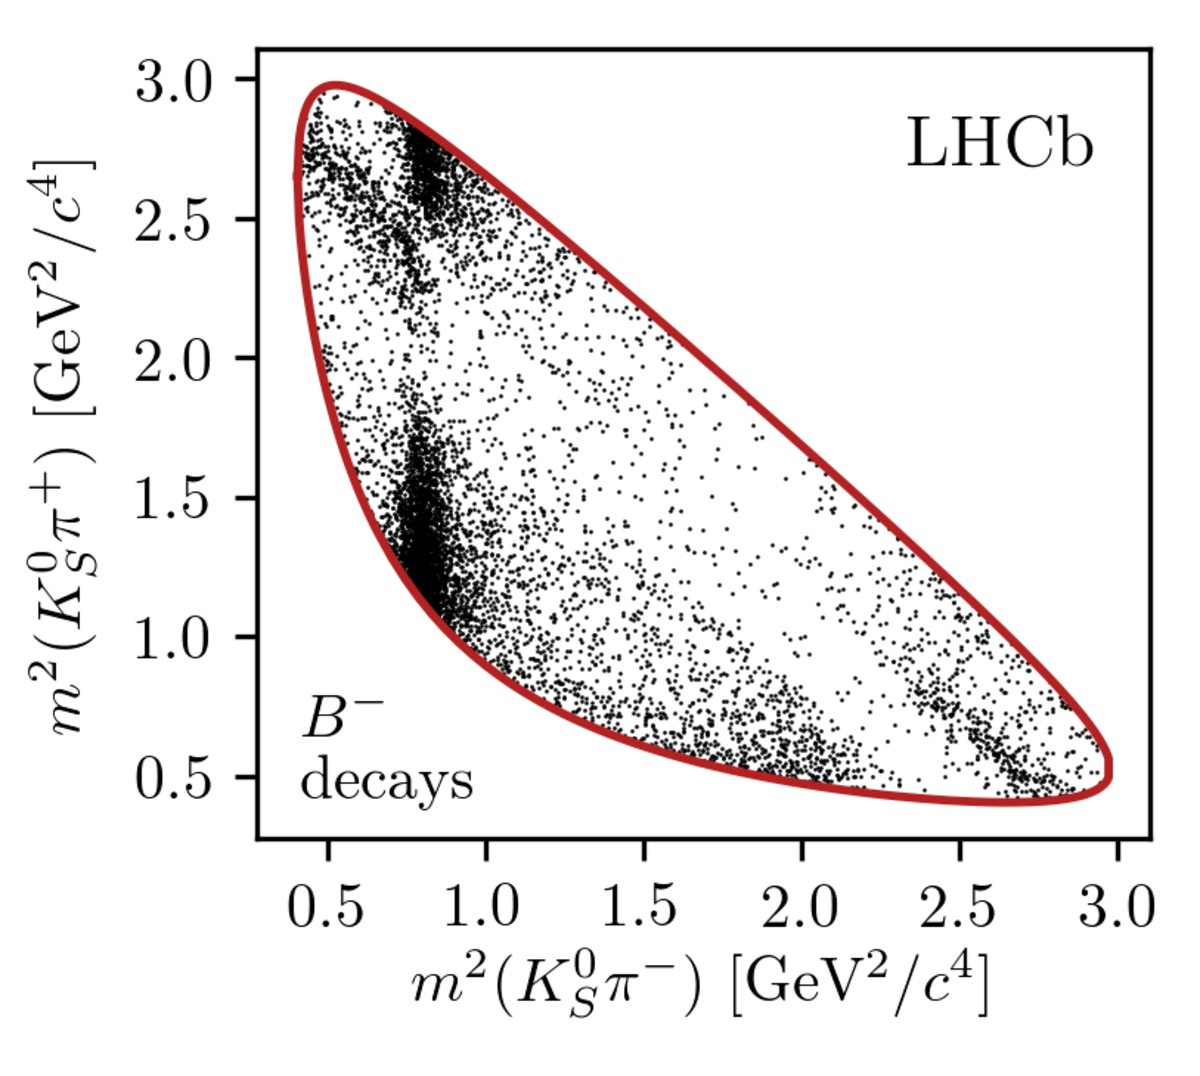
\includegraphics[width = 1.0\textwidth]{Plots/KSpipi_Minus_Dalitz.png}
      \caption*{$B^-\to[K_S^0\pi^+\pi^-]_DK^-$}
    \end{subfigure}%
    \begin{subfigure}{0.5\textwidth}
      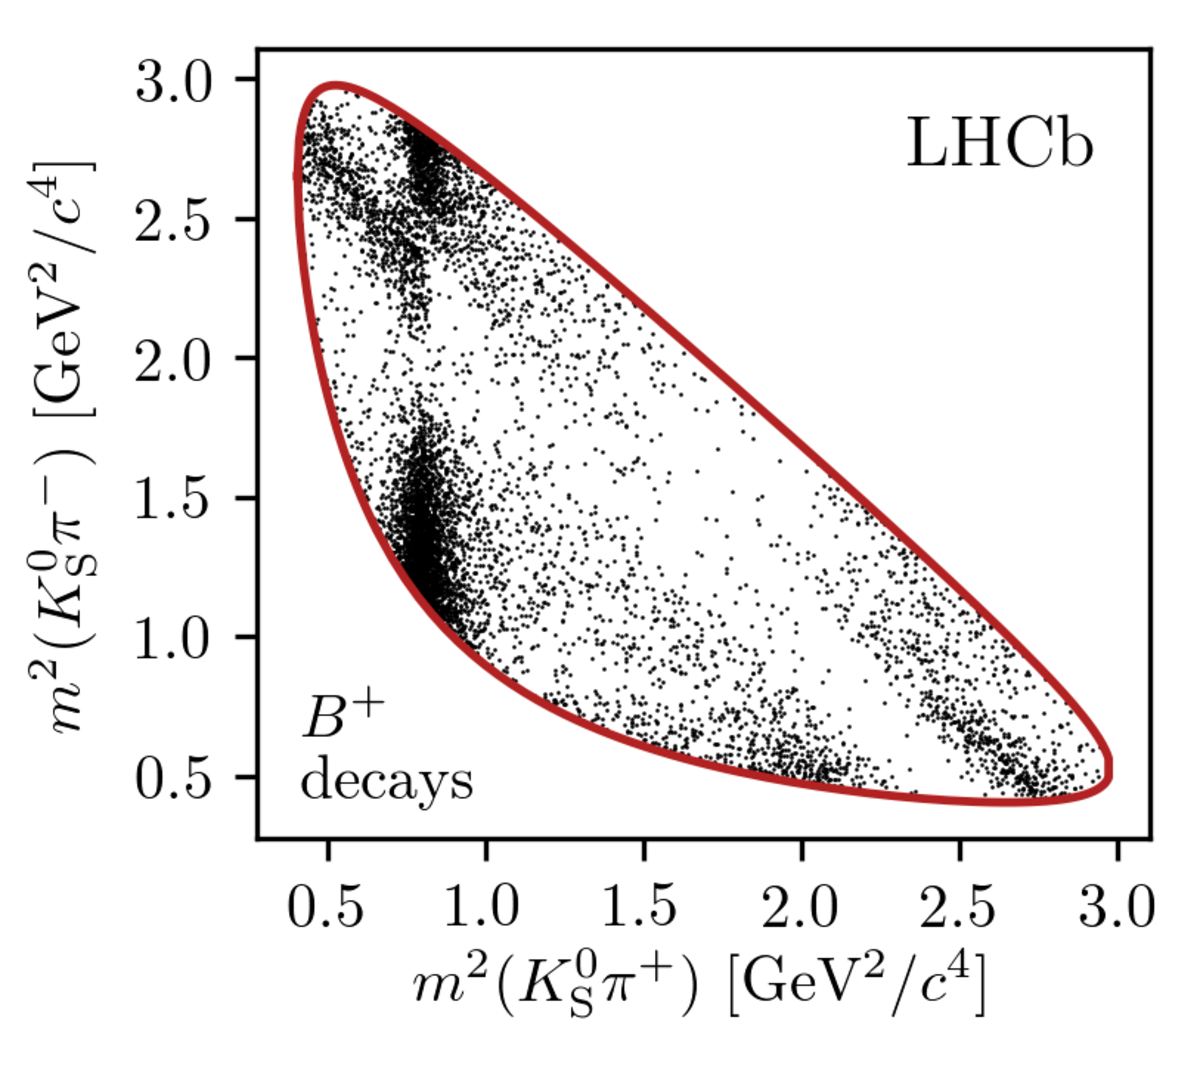
\includegraphics[width = 1.0\textwidth]{Plots/KSpipi_Plus_Dalitz.png}
      \caption*{$B^+\to[K_S^0\pi^+\pi^-]_DK^+$}
    \end{subfigure}
  \end{figure}
  \begin{center}
    \Large Can you find the asymmetries?
  \end{center}
\end{frame}

\section{Binning scheme}
\begin{frame}{Binning scheme}
  \begin{center}
    {\huge Binning scheme}
  \end{center}
\end{frame}

\begin{frame}{Binning scheme}
  \vspace{0.0cm}
  {\Large A binning scheme must satisfy the following:}
  \begin{itemize}
    \item{Minimal dilution of strong phases when integrating over bins}
    \item{Enhance interference between $B^\pm\to D^0K^\pm$ and $B^\pm\to\bar{D^0}K^\pm$}
  \end{itemize}
  \vspace{0.4cm}
  {\Large How to bin a 5-dimensional phase space?}
  \begin{enumerate}
    \item{For each $B^\pm$ candidate, use the amplitude model to calculate}
  \end{enumerate}
  \begin{center}
    {\Large $\frac{\mathcal{A}(D^0)}{\mathcal{A}(\bar{D^0})} = r_De^{i\delta_D}$}
  \end{center}
  \begin{enumerate}
    \setcounter{enumi}{1}
    \setlength\itemsep{0.5em}
    \item{Split $\delta_D$ into uniformly spaced bins}
    \item{Use the symmetry line $r_D = 1$ to separate bin $+i$ from $-i$}
    \item{Optimise the binning scheme by adjusting the bin boundaries in $\delta_D$}
  \end{enumerate}
\end{frame}

\begin{frame}{Binning scheme}
  \begin{figure}
    \centering
    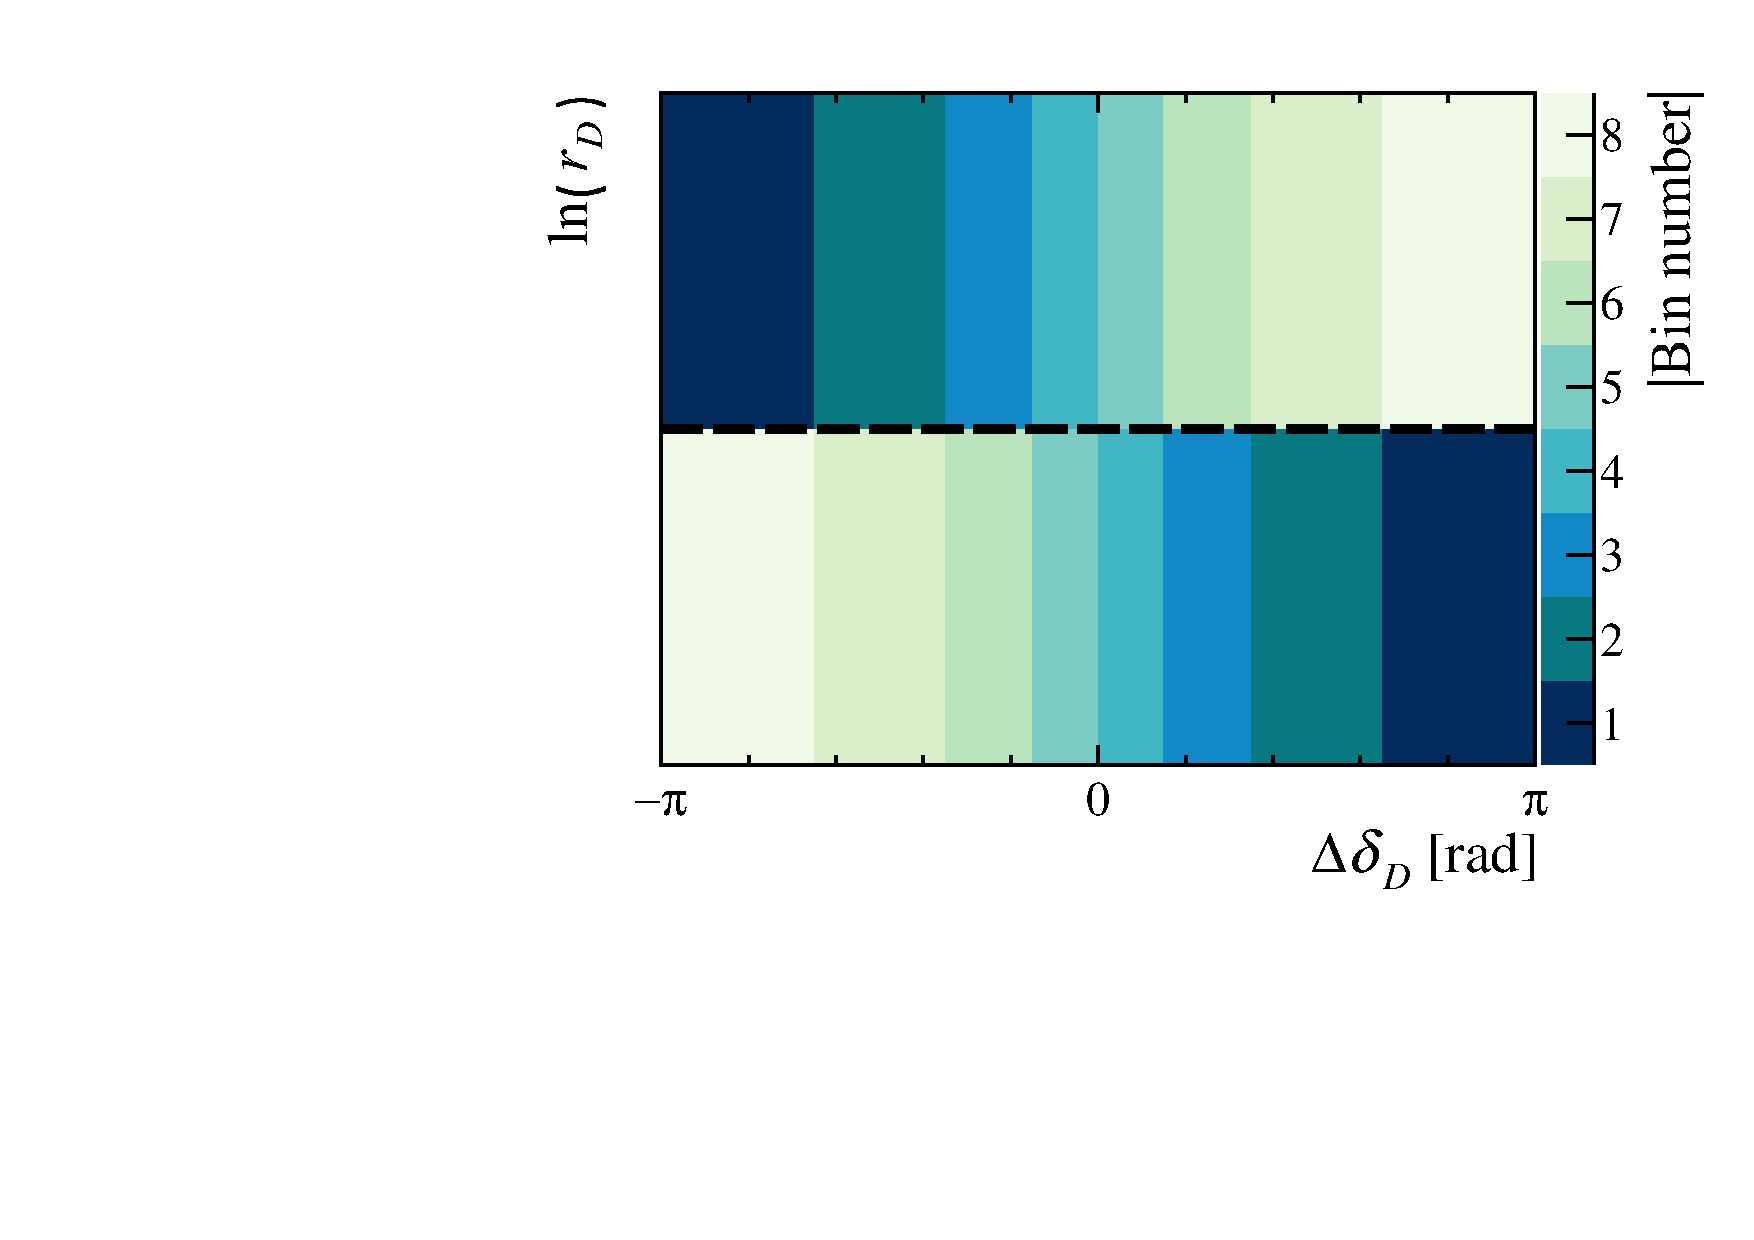
\includegraphics[width = 0.7\textwidth]{Plots/BinningSchemePlot_8Bins.pdf}
  \end{figure}
  \vspace{-1.0cm}
  \begin{center}
    $Q = 0.90$ \\
    Bins $i < 0$ on top, $i > 0$ below
  \end{center}
\end{frame}

\section{Mass fit, \texorpdfstring{$C\!P$}{CP} fit and \texorpdfstring{$\gamma$}{gamma}}
\begin{frame}{Mass fits, $C\!P$ fit and $\gamma$}
  \begin{center}
    {\huge Mass fits, $C\!P$ fit and $\gamma$}
  \end{center}
\end{frame}

\begin{frame}{Mass fits, $C\!P$ fit and $\gamma$}
  \begin{center}
    \large In the end, this analysis is a counting experiment
  \end{center}
  Counting strategy:
  \begin{enumerate}
    \setlength\itemsep{1.0em}
    \item{Perform a ``global fit'' of all $B^\pm$ candidates}
    \item{Fix all shape parameters}
    \item{Sort $B^\pm$ candidates by charge and bins}
    \item{Perform a ``$C\!P$ fit'' simultaneously, but only let bin yields float}
    \item{From the $64$ bin yields, determine $\gamma$ using model-predicted values of $c_i$ and $s_i$}
    \begin{itemize}
      \item{In the future, model-independent measurements of $c_i$ and $s_i$ will become available}
    \end{itemize}
  \end{enumerate}
\end{frame}

\begin{frame}{Mass fits, $C\!P$ fit and $\gamma$}
  \begin{figure}
    \centering
    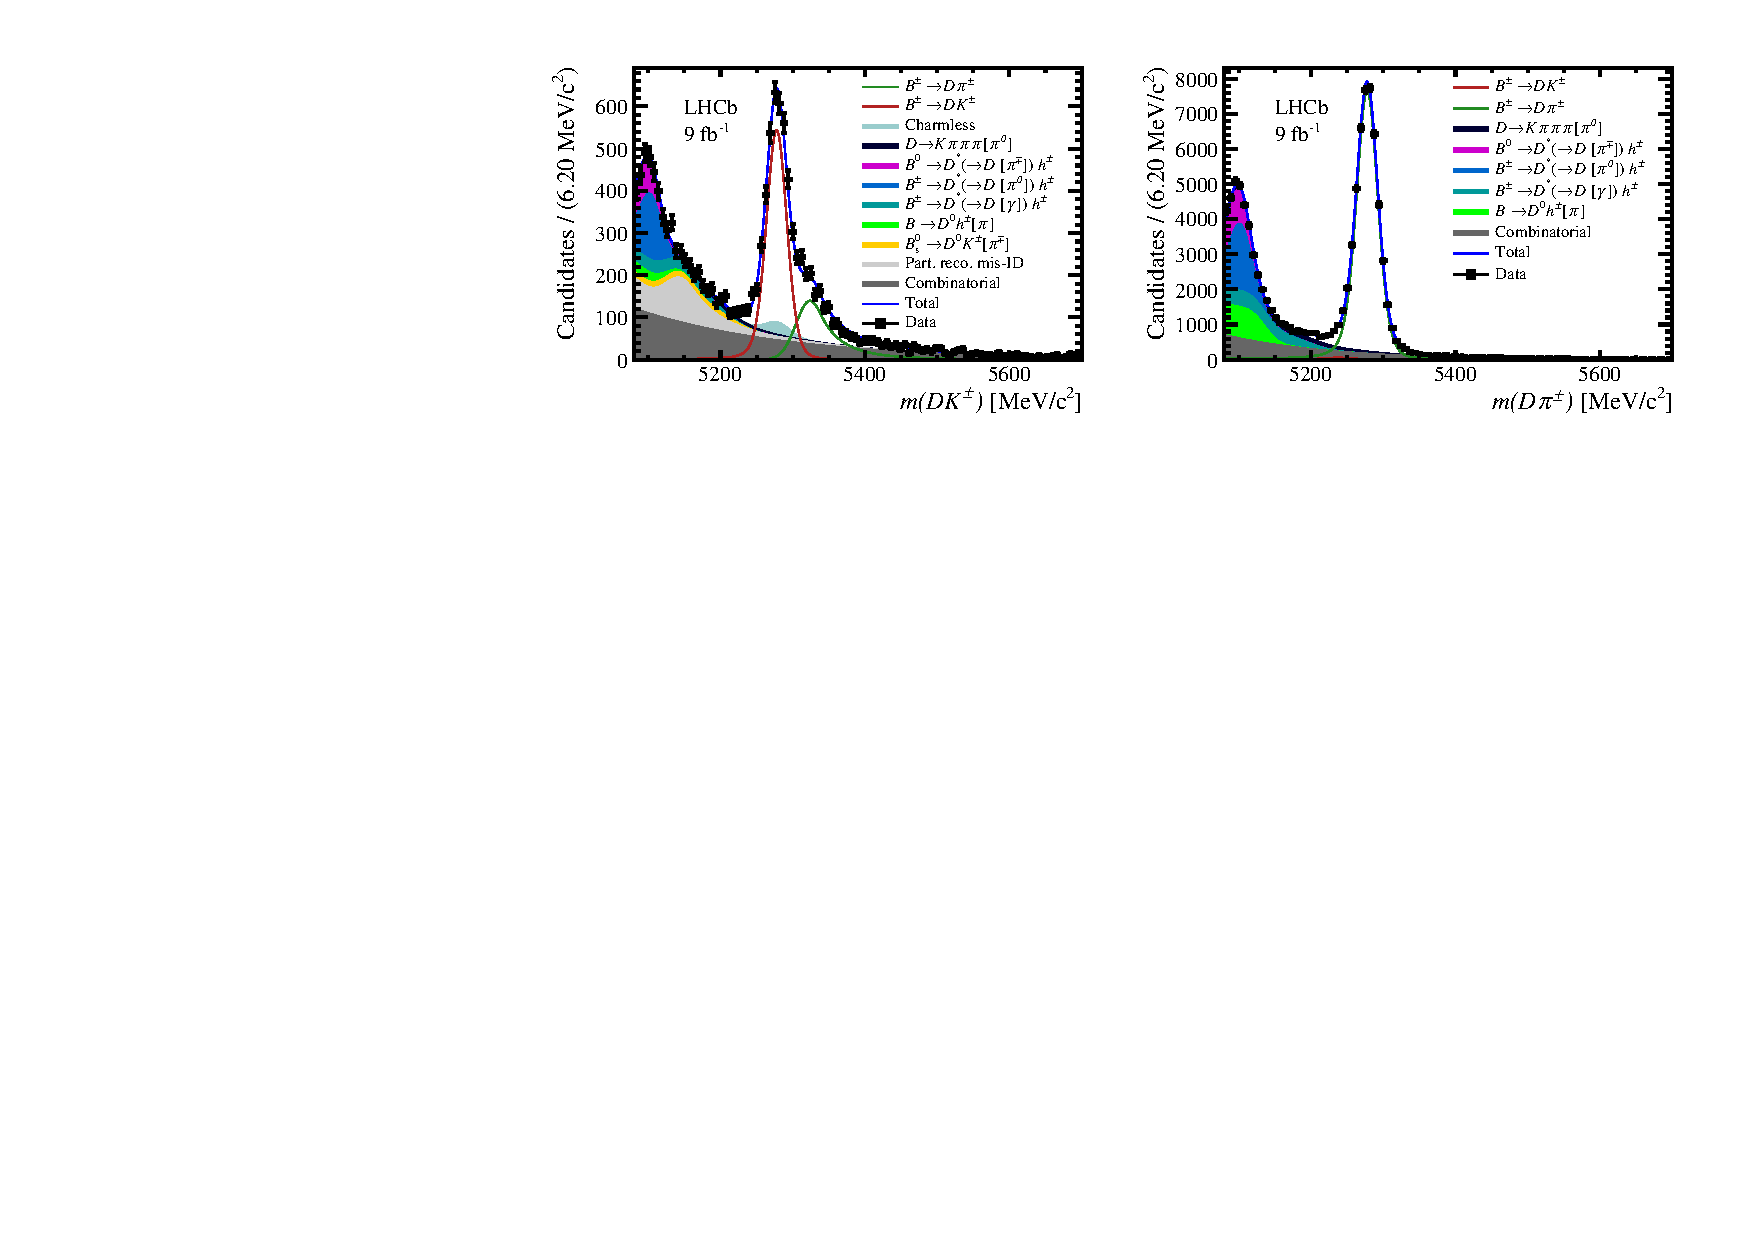
\includegraphics[width = 1.0\textwidth]{Plots/d2kkpipi_fiveL_allDP.pdf}
  \end{figure}
  \begin{center}
    Signal yield:
  \end{center}
  \vspace{-0.3cm}
  \begin{align*}
    B^\pm\to DK^\pm:&\quad \SI{3026(38)}{} \\
    B^\pm\to D\pi^\pm:&\quad \SI{44349(218)}{}
  \end{align*}
\end{frame}

\begin{frame}{Interpretation of $\gamma$}
  \begin{center}
    \Large We can interpret our $C\!P$ observables in terms of the physics parameters $\gamma$, $r_B^{DK}$, $\delta_B^{DK}$, $r_B^{D\pi}$, $\delta_B^{D\pi}$
  \end{center}
  \begin{align*}
    \gamma &= (116^{+12}_{-14})^\circ, \\
    \delta_B^{DK} &= (81^{+14}_{-13})^\circ, \\
    r_B^{DK} &= 0.110^{+0.020}_{-0.020}, \\
    \delta_B^{D\pi} &= (298^{+62}_{-118})^\circ, \\
    r_B^{D\pi} &= 0.0041^{+0.0054}_{-0.0041},
  \end{align*}
  \begin{center}
    \large However, the latest $\gamma$ and charm combination result is:
  \end{center}
  \begin{equation*}
    \gamma = (63.8^{+3.5}_{-3.7})^\circ
  \end{equation*}
  \begin{center}
    \large What went wrong?!
  \end{center}  
\end{frame}

\begin{frame}{Interpretation of $\gamma$}
  \begin{figure}
    \centering
    \begin{overpic}[percent,scale=0.23]{Plots/SpongebobMemeTemplate.png}
      \put(7.5,75){\tiny$\gamma = (116^{+12}_{-14})^\circ$}
    \end{overpic}
  \end{figure}
  \begin{center}
    Do we trust the model predicted $c_i$ and $s_i$, or their uncertainties?
  \end{center}
\end{frame}

\begin{frame}{The $B^\pm\to[K^+K^-\pi^+\pi^-]_DK^\pm$ decay mode}
  \begin{center}
    {\Large There are several reasons why amplitude models \underline{cannot} be trusted}
  \end{center}
  \begin{enumerate}
    \setlength\itemsep{1.0em}
    \item{Amplitude models are just models, which may not reflect reality}
    \item{In fact, the model is fitted to data that knows nothing about $\delta_D(\Phi)$}
    \item{It is \underline{impossible} to assign an objective error to a model!}
  \end{enumerate}
  \vspace{0.5cm}
  \begin{center}
    \large We wish to do a \underline{model independent} measurement\\
    \Large Let's go and measure $c_i$ and $s_i$ at BESIII!
  \end{center}
\end{frame}

\section{Strong phase analysis of \texorpdfstring{$D^0\to K^+K^-\pi^+\pi^-$}{D2KKpipi} at BESIII}
\begin{frame}{Strong phase analysis of $D^0\to K^+K^-\pi^+\pi^-$ at BESIII}
  \begin{center}
    {\huge Strong phase analysis of $D^0\to K^+K^-\pi^+\pi^-$ at BESIII}
  \end{center}
\end{frame}

\begin{frame}{Strong phase analysis of $D^0\to K^+K^-\pi^+\pi^-$ at BESIII}
  \begin{itemize}
    \item{BESIII: Beijing Spectrometer III, a detector at the Beijing Electron-Positron Collider II, located at IHEP}
    \item{$e^+e^-$ collider at the $\psi(3770)\to D^0\bar{D^0}$ threshold}
    \begin{itemize}
      \item{2010-2011: $\SI{3}{\per\femto\barn}$}
      \item{2022: $\SI{5}{\per\femto\barn}$}
      \item{Expect $\SI{20}{\per\femto\barn}$ in total by end of 2024}
    \end{itemize}
  \end{itemize}
  \begin{figure}
    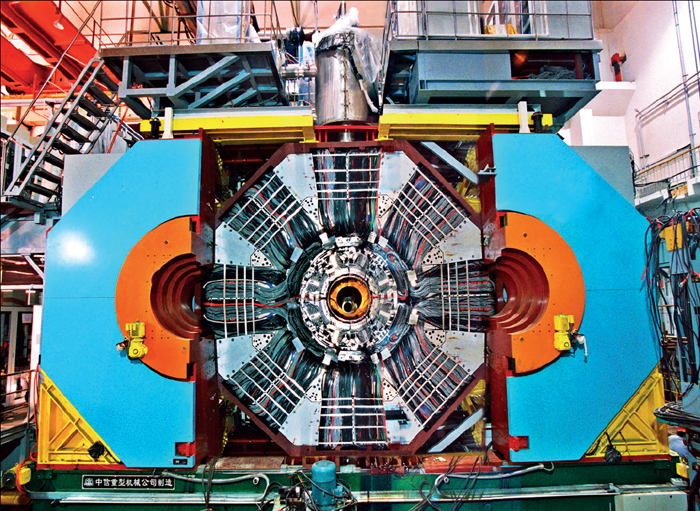
\includegraphics[width = 0.50\textwidth]{Plots/BESIIIDetector.jpg}
  \end{figure}
\end{frame}

\begin{frame}{Strong phase analysis of $D^0\to K^+K^-\pi^+\pi^-$ at BESIII}
  \begin{itemize}
    \item{Double-tag analysis: Reconstruct signal ($KK\pi\pi$) and tag mode}
    \item{$D^0\bar{D^0}$ pair is quantum correlated}
  \end{itemize}
  \begin{figure}[H]
    \centering
    \vspace{-1.5cm}
    \begin{fmffile}{fgraph/fgraph_ee1}
      \setlength{\unitlength}{1cm}
      \begin{fmfgraph*}(8,5)
        \fmfleft{i}
        \fmfright{o}
        \fmflabel{$D^0$}{i}
        \fmflabel{$\bar{D^0}$}{o}
        \fmf{fermion}{w,i}
        \fmf{fermion}{w,o}
        \fmfblob{1cm}{w}
        \fmfv{label=$\psi(3770)$,label.dist=15,label.angle=90}{w}
      \end{fmfgraph*}
    \end{fmffile}
    \vspace{-1.5cm}
  \end{figure}
  \begin{itemize}
    \item{Equivalently, we can consider $D_+D_-$}
    \begin{itemize}
      \item{$D_\pm = \frac{1}{\sqrt{2}}(D^0\pm\bar{D^0})$ are CP eigenstates}
    \end{itemize}
  \end{itemize}
  \begin{figure}[H]
    \centering
    \vspace{-1.5cm}
    \begin{fmffile}{fgraph/fgraph_ee2}
      \setlength{\unitlength}{1cm}
      \begin{fmfgraph*}(8,5)
        \fmfleft{i}
        \fmfright{o}
        \fmflabel{$D_+$}{i}
        \fmflabel{$D_-$}{o}
        \fmf{fermion}{w,i}
        \fmf{fermion}{w,o}
        \fmfblob{1cm}{w}
        \fmfv{label=$\psi(3770)$,label.dist=15,label.angle=90}{w}
      \end{fmfgraph*}
    \end{fmffile}
    \vspace{-1.5cm}
  \end{figure}
  \begin{center}
    The $DD$ pair is \underline{quantum correlated}, spooky action at a distance!
  \end{center}
\end{frame}

\begin{frame}{Strong phase analysis of $D^0\to K^+K^-\pi^+\pi^-$ at BESIII}
  \begin{center}
    Quantum correlation: The $C\!P$ content of the tag can modify the effective branching fraction:
  \end{center}
  \begin{equation*}
    \frac{N^{\rm DT}}{N^{\rm ST}} = \mathcal{B}(D^0\to KK\pi\pi)\big(1\pm c_1\big)
  \end{equation*}
  \begin{figure}
    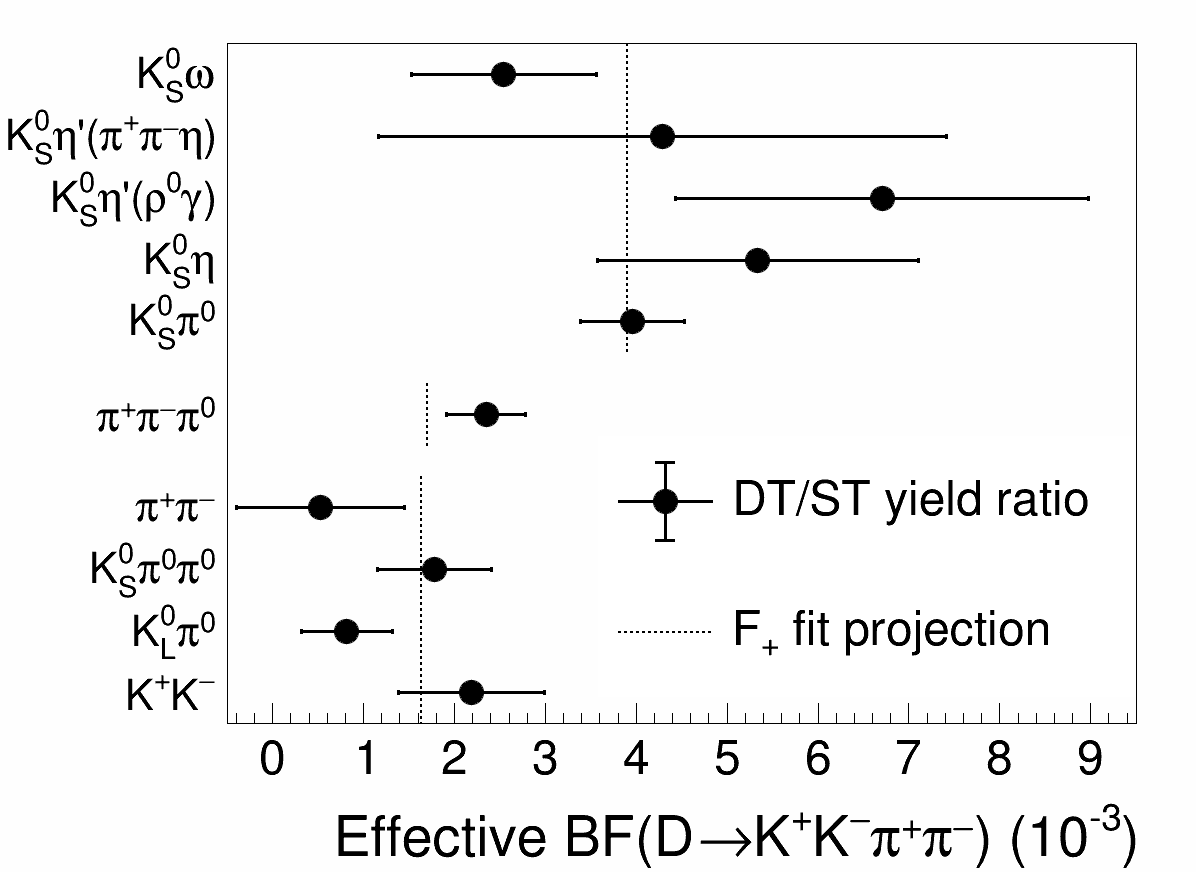
\includegraphics[width = 0.50\textwidth]{Plots/CPeven_fraction_combination_CPtags.png}
    \caption*{\tiny Phys. Rev. D \textbf{107}, 032009}
  \end{figure}
  \vspace{-0.5cm}
  \begin{center}
    $c_1$ is the cosine of the strong phase, averaged over the \underline{whole} phase space
  \end{center}
\end{frame}

\begin{frame}{Strong phase analysis of $D^0\to K^+K^-\pi^+\pi^-$ at BESIII}
  \begin{center}
    Our next task is to change the phase space inclusive analysis,
  \end{center}
  \vspace{-0.5cm}
  \begin{align*}
    \frac{N^{\rm DT}}{N^{\rm ST}} =& \mathcal{B}(D^0\to KK\pi\pi)\quad\textnormal{(flavour tag)} \\
    \frac{N^{\rm DT}}{N^{\rm ST}} =& \mathcal{B}(D^0\to KK\pi\pi)\big(1\pm c_1\big)\quad\textnormal{(CP tag)}
  \end{align*}
  \vspace{-1.0cm}
  \begin{center}
    into a binned phase space analysis:
  \end{center}
  \vspace{-0.6cm}
  \begin{align*}
    \frac{N^{\rm DT}_i}{N^{\rm ST}} =& \mathcal{B}(D^0\to KK\pi\pi)F_i\quad\textnormal{(flavour tag)} \\
    \frac{N^{\rm DT}_i}{N^{\rm ST}} =& \mathcal{B}(D^0\to KK\pi\pi)\big(F_i + \bar{F_i} \pm 2\sqrt{F_i\bar{F_i}}c_i\big)\quad\textnormal{(CP tag)}
  \end{align*}
  \vspace{-0.6cm}
  \begin{enumerate}
    \item{$F_i$: Measure using flavour tags}
    \item{$c_i$: Determine from asymmetry of $C\!P$ even and odd tags}
    \item{$s_i$: Analogous to $c_i$, but requires binning of tag mode}
  \end{enumerate}
  \vspace{-7.0cm}
  \begin{center}
    \phantom{\rotatebox{45}{\Huge\colorbox{white}{\framebox{Work in progress!}}}}
  \end{center}
\end{frame}

\begin{frame}{Strong phase analysis of $D^0\to K^+K^-\pi^+\pi^-$ at BESIII}
  \begin{center}
    Our next task is to change the phase space inclusive analysis,
  \end{center}
  \vspace{-0.5cm}
  \begin{align*}
    \frac{N^{\rm DT}}{N^{\rm ST}} =& \mathcal{B}(D^0\to KK\pi\pi)\quad\textnormal{(flavour tag)} \\
    \frac{N^{\rm DT}}{N^{\rm ST}} =& \mathcal{B}(D^0\to KK\pi\pi)\big(1\pm c_1\big)\quad\textnormal{(CP tag)}
  \end{align*}
  \vspace{-1.0cm}
  \begin{center}
    into a binned phase space analysis:
  \end{center}
  \vspace{-0.6cm}
  \begin{align*}
    \frac{N^{\rm DT}_i}{N^{\rm ST}} =& \mathcal{B}(D^0\to KK\pi\pi)F_i\quad\textnormal{(flavour tag)} \\
    \frac{N^{\rm DT}_i}{N^{\rm ST}} =& \mathcal{B}(D^0\to KK\pi\pi)\big(F_i + \bar{F_i} \pm 2\sqrt{F_i\bar{F_i}}c_i\big)\quad\textnormal{(CP tag)}
  \end{align*}
  \vspace{-0.6cm}
  \begin{enumerate}
    \item{$F_i$: Measure using flavour tags}
    \item{$c_i$: Determine from asymmetry of $C\!P$ even and odd tags}
    \item{$s_i$: Analogous to $c_i$, but requires binning of tag mode}
  \end{enumerate}
  \vspace{-7.0cm}
  \begin{center}
    \rotatebox{45}{\Huge\colorbox{white}{\framebox{Work in progress!}}}
  \end{center}
\end{frame}

\section{Summary and conclusion}
\begin{frame}{Summary and conclusion}
  \begin{enumerate}
    \setlength\itemsep{1.0em}
    \item{I have presented the first model-independent measurement of $\gamma$ using $B^\pm\to[K^+K^-\pi^+\pi^-]_Dh^\pm$}
    \item{The optimised binning scheme, developed with an amplitude model, successfully identified regions with large, local $C\!P$ asymmetries}
  \end{enumerate}
  \begin{columns}[onlytextwidth]
    \begin{column}{0.5\textwidth}
      \centering
      \begin{enumerate}
        \setcounter{enumi}{2}
        \setlength\itemsep{1.0em}
        \item{However, amplitude model predictions of $\delta_D$ \underline{should not be trusted}}
        \item{$3\sigma$ tension with world average}
      \end{enumerate}
    \end{column}
    \begin{column}{0.5\textwidth}
      \begin{figure}
        \begin{overpic}[percent,scale=0.2]{Plots/SpongebobAmplitudeModel.png}
          \put(58,64){\small Making binning}
          \put(58,56){\small scheme with}
          \put(58,48){\small amplitude model}
          \put(58,30){\small Predicting strong}
          \put(58,22){\small phases with}
          \put(58,14){\small amplitude model}
        \end{overpic}
      \end{figure}
    \end{column}
  \end{columns}
  \begin{enumerate}
    \setlength\itemsep{1.0em}
    \setcounter{enumi}{4}
    \item{External inputs from charm factories, such as BESIII, are crucial to constrain charm strong phases}
  \end{enumerate}
\end{frame}

\begin{frame}{Summary and conclusion}
  \begin{center}
    {\huge Thanks for your attention!}
  \end{center}
\end{frame}

\section{Backup slides}
\begin{frame}{Backup slides}
  \begin{center}
    {\huge Backup slides}
  \end{center}
\end{frame}

\begin{frame}{Event selection}
  \begin{center}
    {\huge Event selection}
  \end{center}
\end{frame}

\begin{frame}{Event selection}
  \begin{center}
    \Large Decay topology
  \end{center}
  \vspace{0.5cm}
  \begin{columns}
    \begin{column}{0.4\textwidth}
      Look for:
      \begin{enumerate}
        \item{5 charged tracks}
        \item{Displaced $B$ vertex}
        \item{1 bachelor track with good PID information}
        \item{Displaced $D$ vertex with invariant mass within $\SI{25}{\mega\eV}$ of the $D^0$ mass}
      \end{enumerate}
    \end{column}
    \begin{column}{0.6\textwidth}
      \begin{figure}[H]
        \centering
        \begin{fmffile}{fgraph/fgraph_DecayTopology}
          \setlength{\unitlength}{0.4cm}
          \begin{fmfgraph*}(9,9)
            \fmfleft{i1,i2,i3}
            \fmfv{decor.shape=circle,decor.filled=shaded,decor.size=0.2w,label=IP,label.angle=180,label.dist=0.5cm}{i1}
            \fmfright{o1,o2,o3,o4,o5}
            \fmflabel{$\pi^+$}{o1}
            \fmflabel{$\pi^-$}{o2}
            \fmflabel{$K^+$}{o3}
            \fmflabel{$K^-$}{o4}
            \fmflabel{$K^-$}{o5}
            \fmf{phantom,tension=1.5}{i3,v1}
            \fmf{dashes,tension=2.5}{i1,v1}
            \fmfv{decor.shape=circle,decor.filled=shaded,decor.size=0.15w,label=$B^-$,label.angle=110,label.dist=0.5cm}{v1}
            \fmf{plain}{v1,o5}
            \fmf{dashes,tension=1.5}{v1,v2}
            \fmfv{decor.shape=circle,decor.filled=shaded,decor.size=0.15w,label=$D$,label.angle=-110,label.dist=0.5cm}{v2}
            \fmf{plain}{v2,o1}
            \fmf{plain}{v2,o2}
            \fmf{plain}{v2,o3}
            \fmf{plain}{v2,o4}
          \end{fmfgraph*}
        \end{fmffile}
        \vspace{0.5cm}
      \end{figure}
    \end{column}
  \end{columns}
\end{frame}

\begin{frame}{Event selection}
  \begin{center}
    \large Offline selection has 3 stages
  \end{center}
  Initial cuts:
  \begin{enumerate}
    \item{Invariant $D$ and $B$ mass cuts}
    \item{Momentum and RICH requirements}
  \end{enumerate}
  Boosted Decision Tree (BDT)
  \begin{itemize}
    \item{Signal sample: Simulation samples}
    \item{Background sample: Upper $B$ mass sideband}
    \item{28 variables describing kinematics, impact parameters, vertex quality}
  \end{itemize}
  Final selection
  \begin{enumerate}
    \item{$D$ Flight distance}
    \item{Particle Identification of bachelor}
    \item{$K_S^0$ veto}
  \end{enumerate}
\end{frame}

\begin{frame}{Event selection}
  \begin{figure}
    \centering
    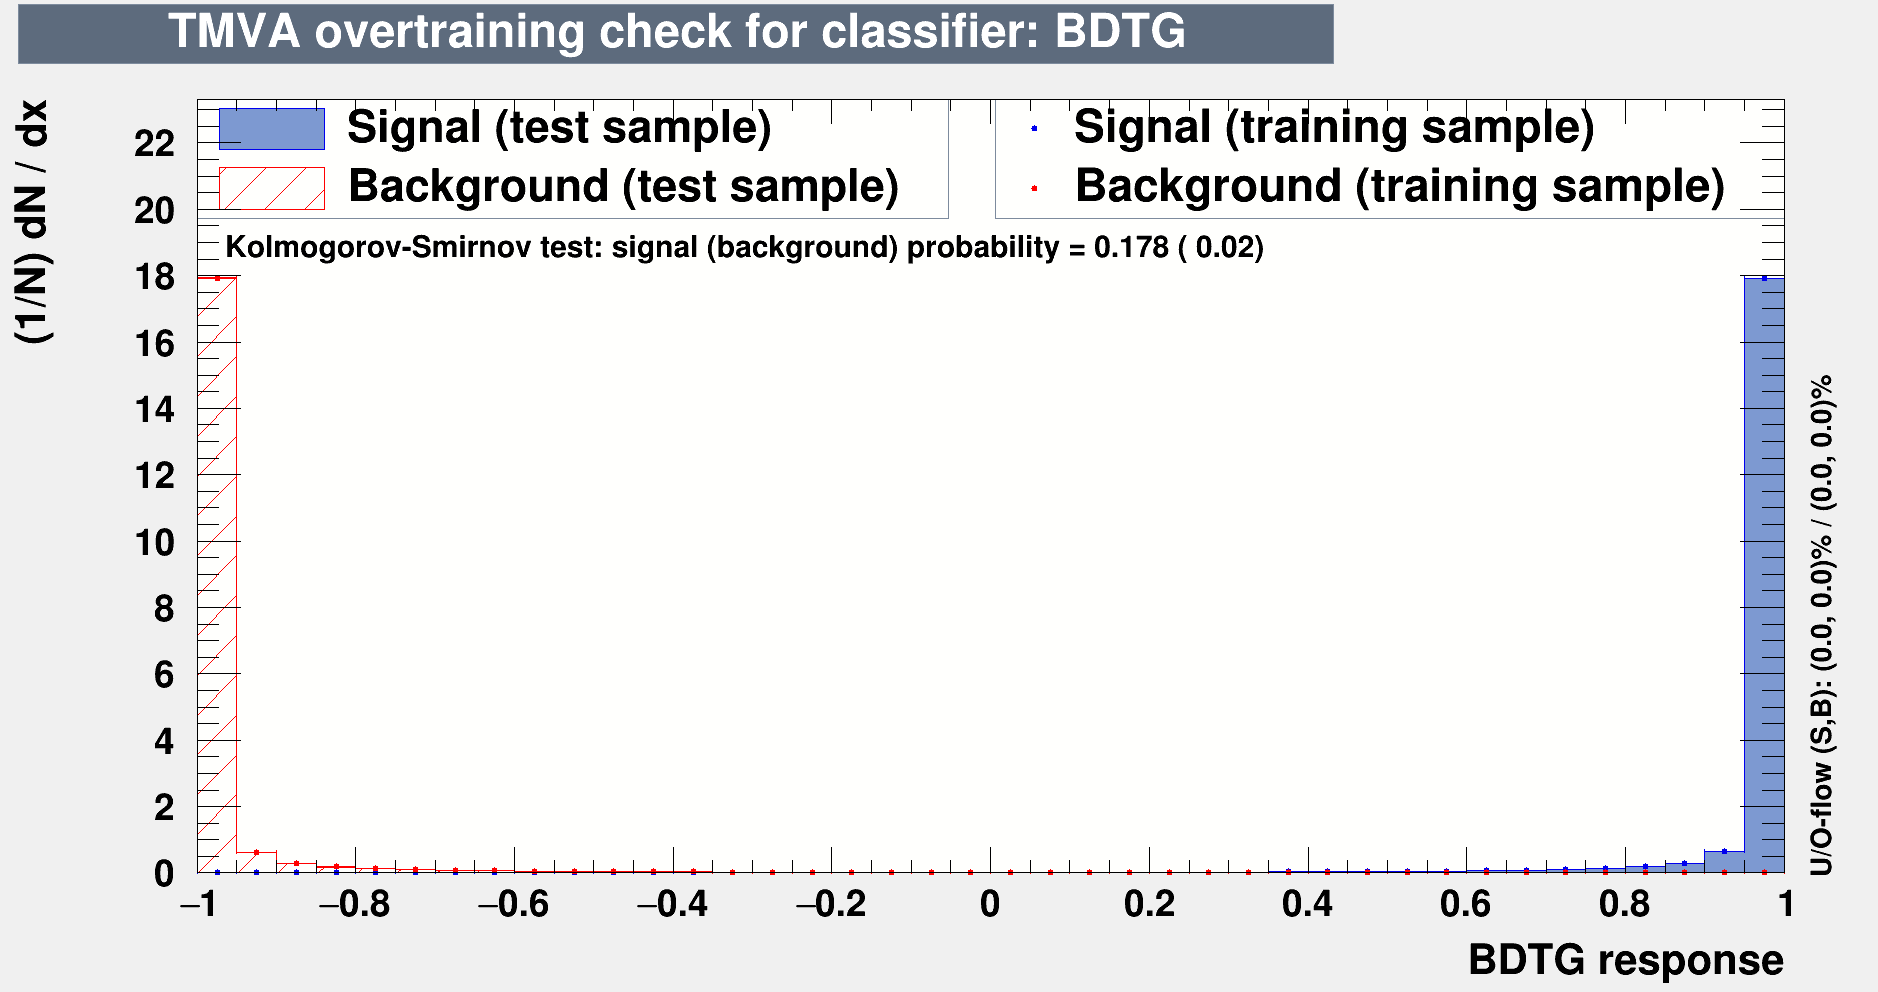
\includegraphics[width = 1.0\textwidth]{Plots/overtrain_BDTG.png}
  \end{figure}
  \begin{center}
    BDT is highly efficient at rejecting combinatorial background
  \end{center}
\end{frame}

\begin{frame}{Event selection}
  \begin{figure}
    \centering
    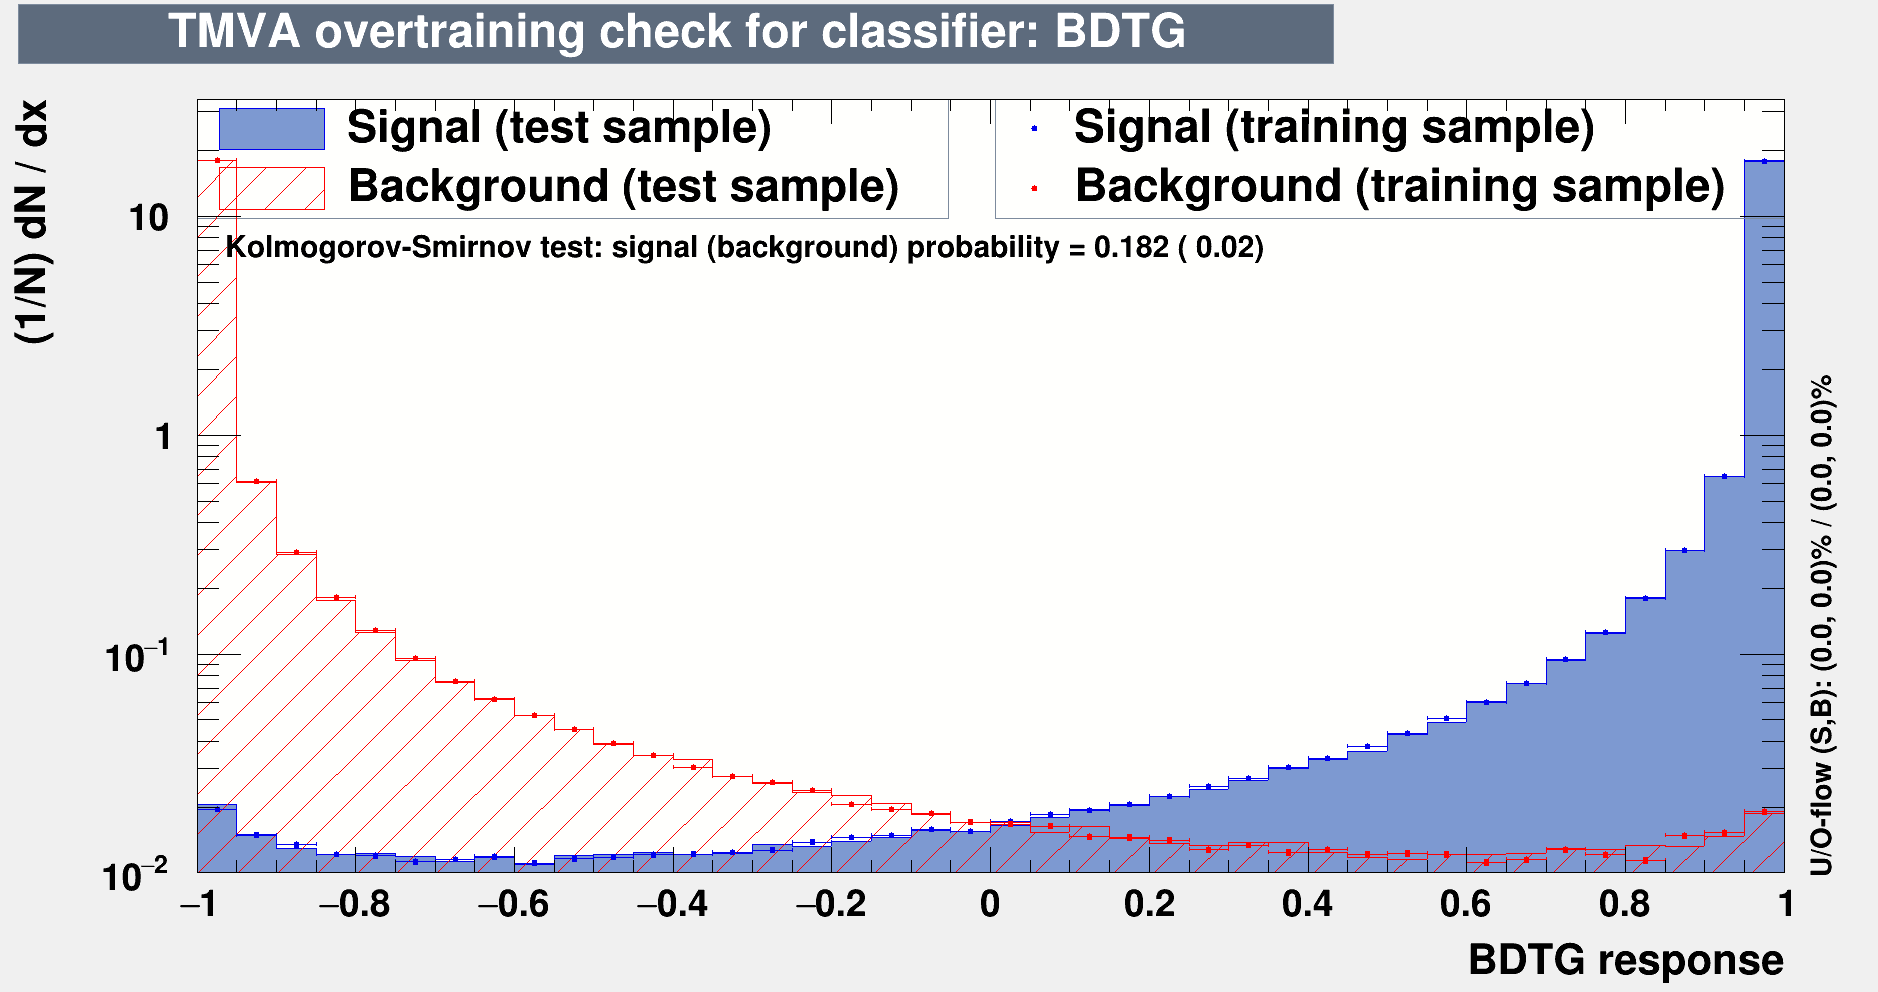
\includegraphics[width = 1.0\textwidth]{Plots/overtrain_BDTG_log.png}
  \end{figure}
  \begin{center}
    Very important, combinatorial background is large in multi-body decays
  \end{center}
\end{frame}

\begin{frame}{Event selection}
  \begin{figure}
    \centering
    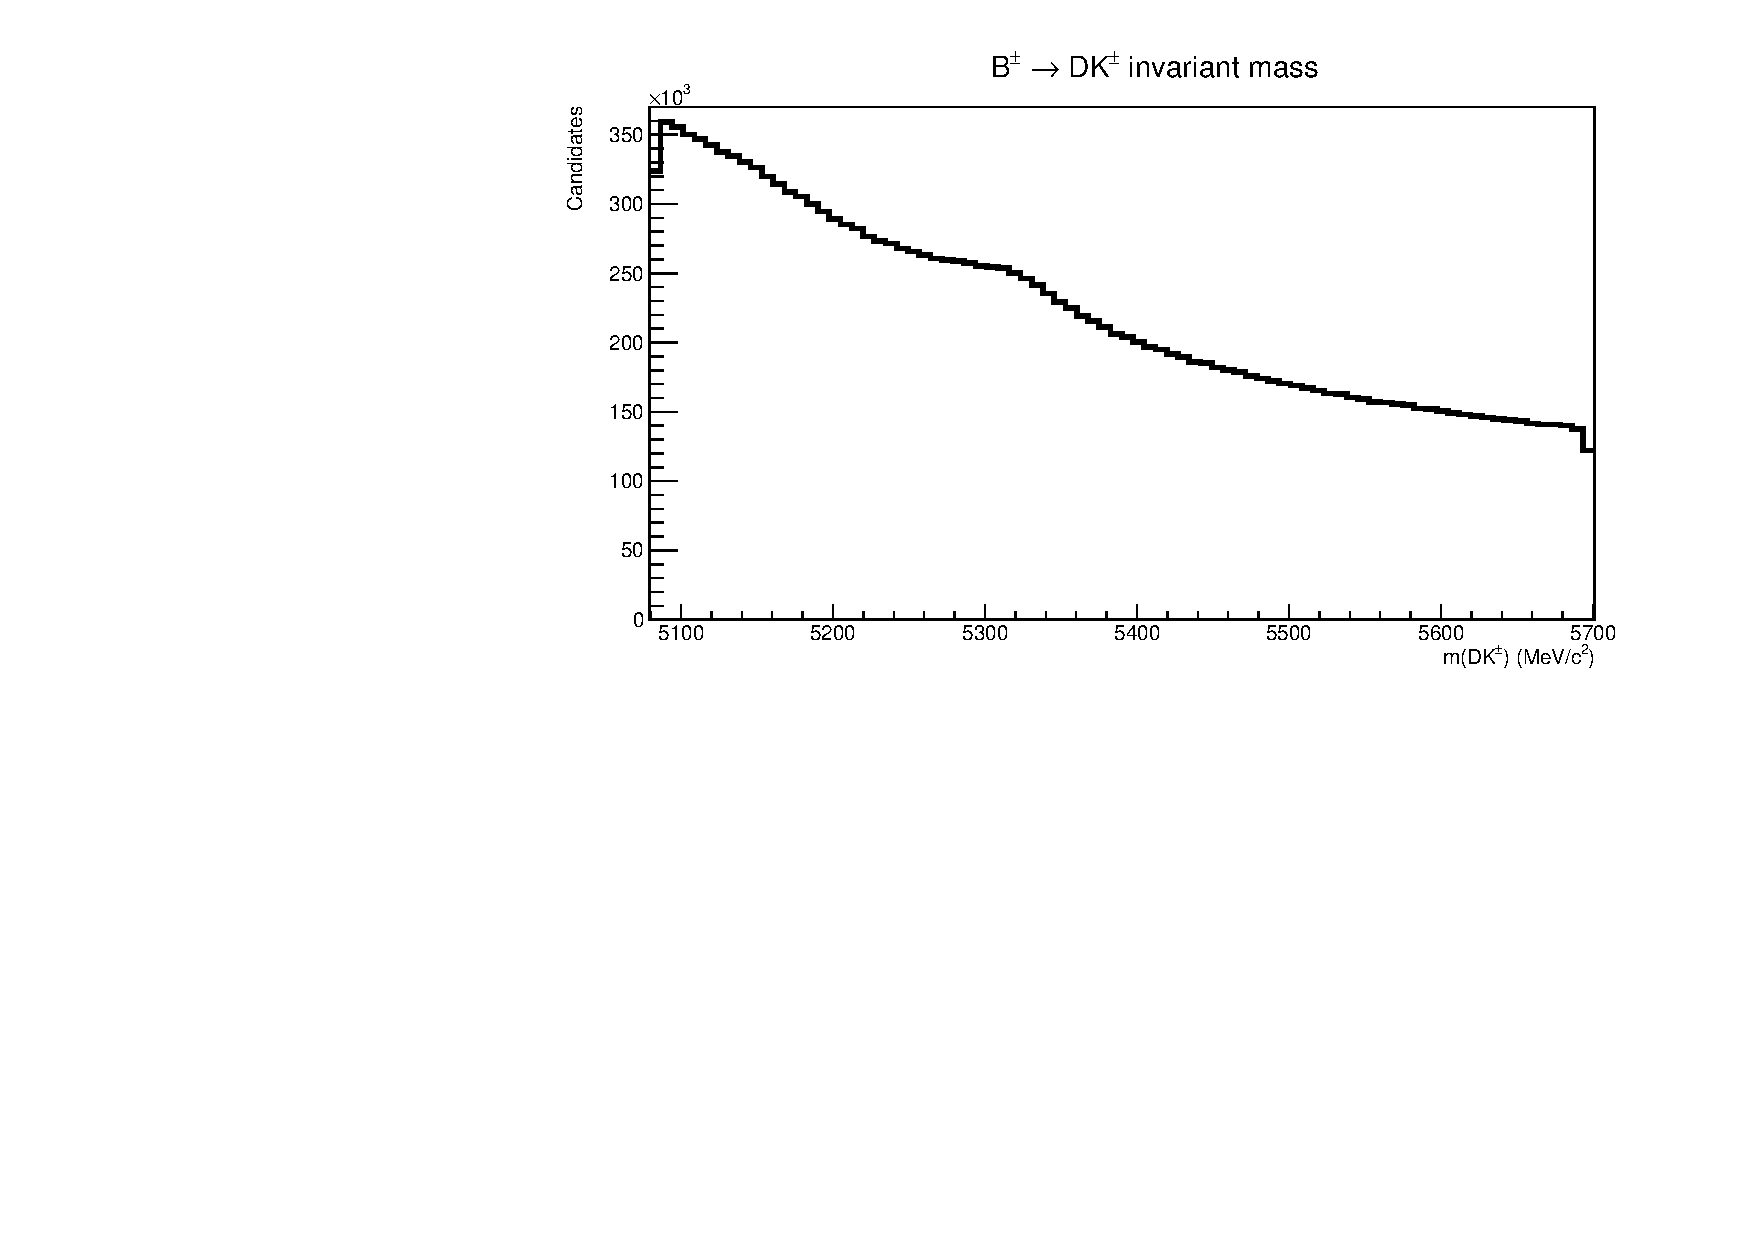
\includegraphics[width = 1.0\textwidth]{Plots/BmassStripping.pdf}
  \end{figure}
  \begin{center}
    The invariant $B$ mass, after online selection, show no visible signal...
  \end{center}
\end{frame}

\begin{frame}{Event selection}
  \begin{figure}
    \centering
    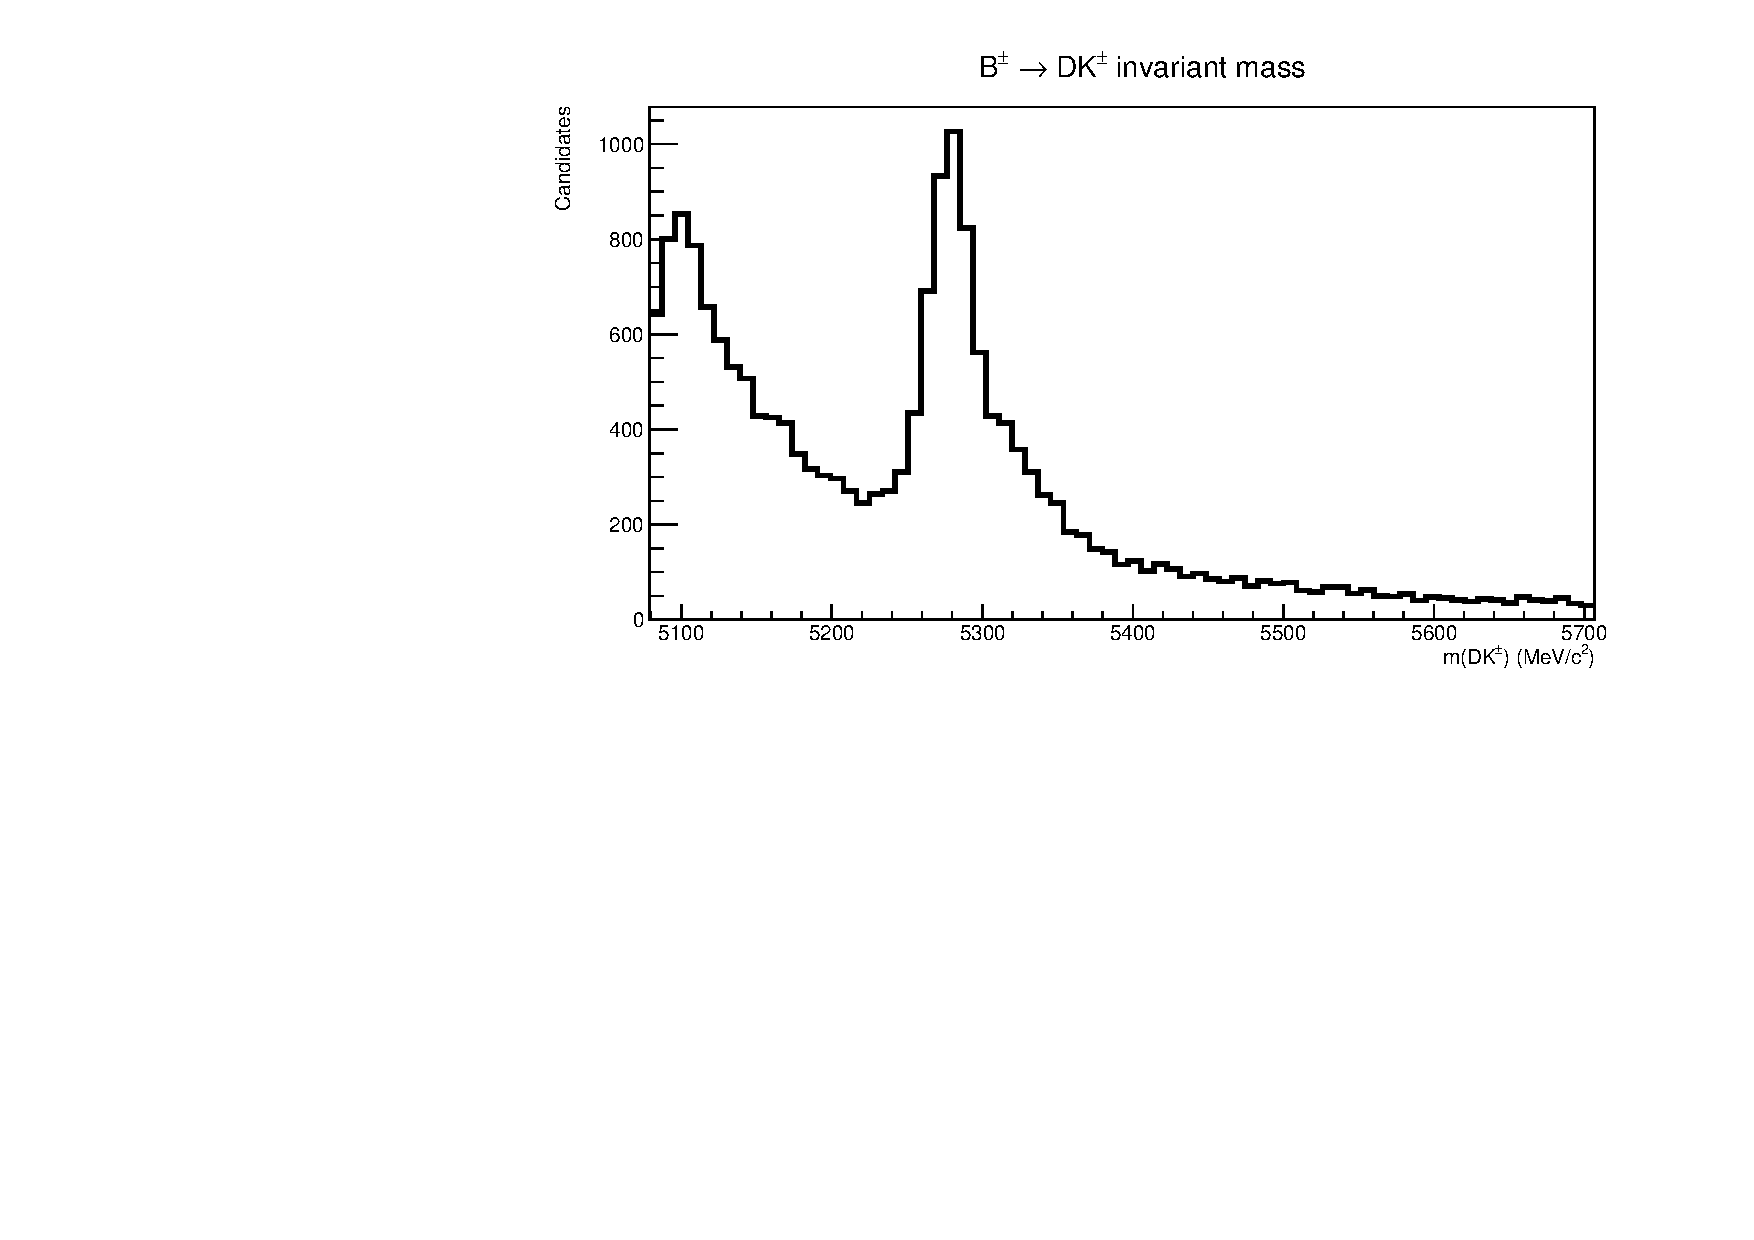
\includegraphics[width = 1.0\textwidth]{Plots/BmassFinalSelection.pdf}
  \end{figure}
  \begin{center}
    ... but the BDT does a great job cleaning this up!
  \end{center}
\end{frame}

\end{document}
